\documentclass[dvips, lscape]{foils}
%\documentclass[dvips, french]{slides}
\textwidth 18.5cm
\textheight 25cm 
\topmargin -1cm 
\oddsidemargin  -1cm 
\evensidemargin  -1cm

% Maths
\usepackage{amsfonts, amsmath, amssymb}

\newcommand{\coefbin}[2]{\left( 
    \begin{array}{c} #1 \\ #2 \end{array} 
  \right)}
\newcommand{\Bcal}{\mathcal{B}}
\newcommand{\Ccal}{\mathcal{C}}
\newcommand{\Dcal}{\mathcal{D}}
\newcommand{\Ecal}{\mathcal{E}}
\newcommand{\Mcal}{\mathcal{M}}
\newcommand{\Ncal}{\mathcal{N}}
\newcommand{\Pcal}{\mathcal{P}}
\newcommand{\Lcal}{\mathcal{L}}
\newcommand{\Tcal}{\mathcal{T}}
\newcommand{\Ucal}{\mathcal{U}}
\newcommand{\lFDR}{\ell FDR}
\newcommand{\alphabf}{\mbox{\mathversion{bold}{$\alpha$}}}
\newcommand{\betabf}{\mbox{\mathversion{bold}{$\beta$}}}
\newcommand{\gammabf}{\mbox{\mathversion{bold}\newcommand{\psibf}{\mbox{\mathversion{bold}{$\psi$}}}
{$\gamma$}}}
\newcommand{\mubf}{\mbox{\mathversion{bold}{$\mu$}}}
\newcommand{\psibf}{\mbox{\mathversion{bold}{$\psi$}}}
\newcommand{\Sigmabf}{\mbox{\mathversion{bold}{$\Sigma$}}}
\newcommand{\taubf}{\mbox{\mathversion{bold}{$\tau$}}}
\newcommand{\Hbf}{{\bf H}}
\newcommand{\Ibf}{{\bf I}}
\newcommand{\Sbf}{{\bf S}}
\newcommand{\mbf}{{\bf m}}
\newcommand{\ubf}{{\bf u}}
\newcommand{\vbf}{{\bf v}}
\newcommand{\xbf}{{\bf x}}
\newcommand{\Xbf}{{\bf X}}
\newcommand{\Esp}{{\mathbb E}}
\newcommand{\Var}{{\mathbb V}}
\newcommand{\Cov}{{\mathbb C}\mbox{ov}}
\newcommand{\Ibb}{{\mathbb I}}
\newcommand{\Rbb}{\mathbb{R}}

% sommes
\newcommand{\sumk}{\sum_k}
\newcommand{\sumt}{\sum_{t \in I_k}}
\newcommand{\sumth}{\sum_{t=t_{k-1}^{(h)}+1}^{t_k^{(h)}}}
\newcommand{\sump}{\sum_{p=1}^{P}}
\newcommand{\suml}{\sum_{\ell=1}^{P}}
\newcommand{\sumtau}{\sum_k \hat{\tau}_{kp}}

% Couleur et graphiques
\usepackage{color}
\usepackage{graphics}
\usepackage{epsfig} 
\usepackage{pstcol}

% Texte
\usepackage{lscape}
\usepackage{../../../../Latex/fancyheadings, rotating, enumerate}
%\usepackage[french]{babel}
\usepackage[latin1]{inputenc}
\definecolor{darkgreen}{cmyk}{0.5, 0, 0.5, 0.5}
\definecolor{orange}{cmyk}{0, 0.6, 0.8, 0}
\definecolor{jaune}{cmyk}{0, 0.5, 0.5, 0}
\newcommand{\textblue}[1]{\textcolor{blue}{#1}}
\newcommand{\textred}[1]{\textcolor{red}{#1}}
\newcommand{\textgreen}[1]{\textcolor{green}{ #1}}
\newcommand{\textlightgreen}[1]{\textcolor{green}{#1}}
%\newcommand{\textgreen}[1]{\textcolor{darkgreen}{#1}}
\newcommand{\textorange}[1]{\textcolor{orange}{#1}}
\newcommand{\textyellow}[1]{\textcolor{yellow}{#1}}
\newcommand{\refer}[2]{{\sl #1}}

% Sections
%\newcommand{\chapter}[1]{\centerline{\LARGE \textblue{#1}}}
% \newcommand{\section}[1]{\centerline{\Large \textblue{#1}}}
% \newcommand{\subsection}[1]{\noindent{\Large \textblue{#1}}}
% \newcommand{\subsubsection}[1]{\noindent{\large \textblue{#1}}}
% \newcommand{\paragraph}[1]{\noindent {\textblue{#1}}}
% Sectionsred
 \newcommand{\chapter}[1]{
   \addtocounter{chapter}{1}
   \setcounter{section}{0}
   \setcounter{subsection}{0}
   {\centerline{\LARGE \textblue{\arabic{chapter} - #1}}}
   }
 \newcommand{\section}[1]{
   \addtocounter{section}{1}
   \setcounter{subsection}{0}
   {\centerline{\Large \textblue{\arabic{chapter}.\arabic{section} - #1}}}
   }
% \newcommand{\subsection}[1]{
%   \addtocounter{subsection}{1}
%   {\noindent{\large \textblue{\arabic{chapter}.\arabic{section}.\arabic{subsection} - #1}}}
%   }
%\newcommand{\chapter}[1]{
%  {\centerline{\LARGE \textblue{#1}}}
%  }
%\newcommand{\section}[1]{
%  {\centerline{\Large \textblue{#1}}}
%  }
\newcommand{\subsection}[1]{
  {\noindent{\large \textblue{#1}}}
  }
\newcommand{\paragraph}[1]{\noindent{\textblue{#1}}}

%%%%%%%%%%%%%%%%%%%%%%%%%%%%%%%%%%%%%%%%%%%%%%%%%%%%%%%%%%%%%%%%%%%%%%
%%%%%%%%%%%%%%%%%%%%%%%%%%%%%%%%%%%%%%%%%%%%%%%%%%%%%%%%%%%%%%%%%%%%%%
%%%%%%%%%%%%%%%%%%%%%%%%%%%%%%%%%%%%%%%%%%%%%%%%%%%%%%%%%%%%%%%%%%%%%%
%%%%%%%%%%%%%%%%%%%%%%%%%%%%%%%%%%%%%%%%%%%%%%%%%%%%%%%%%%%%%%%%%%%%%%
\begin{document}
%%%%%%%%%%%%%%%%%%%%%%%%%%%%%%%%%%%%%%%%%%%%%%%%%%%%%%%%%%%%%%%%%%%%%%
%%%%%%%%%%%%%%%%%%%%%%%%%%%%%%%%%%%%%%%%%%%%%%%%%%%%%%%%%%%%%%%%%%%%%%
%%%%%%%%%%%%%%%%%%%%%%%%%%%%%%%%%%%%%%%%%%%%%%%%%%%%%%%%%%%%%%%%%%%%%%
%%%%%%%%%%%%%%%%%%%%%%%%%%%%%%%%%%%%%%%%%%%%%%%%%%%%%%%%%%%%%%%%%%%%%%
\landscape
\newcounter{chapter}
\newcounter{section}
\newcounter{subsection}
\setcounter{chapter}{0}
\headrulewidth 0pt 
\pagestyle{fancy} 
\cfoot{}
\rfoot{\begin{rotate}{90}{
      \hspace{1cm} \tiny Robin: Statistical analysis of biochip data}
  \end{rotate}}
\rhead{\begin{rotate}{90}{
      \hspace{-.5cm} \tiny \thepage
      }\end{rotate}}

%%%%%%%%%%%%%%%%%%%%%%%%%%%%%%%%%%%%%%%%%%%%%%%%%%%%%%%%%%%%%%%%%%%%%%
%%%%%%%%%%%%%%%%%%%%%%%%%%%%%%%%%%%%%%%%%%%%%%%%%%%%%%%%%%%%%%%%%%%%%%
\begin{center}
  \textblue{\LARGE Statistical analysis of biochip data}

   \vspace{1cm}
   {\large S. Robin} \\
   robin@inapg.inra.fr

   {UMR INA-PG / ENGREF / INRA, Paris} \\
   {Math�matique et Informatique Appliqu�es}
   
    \vspace{0.5cm}
    {European Workshop on Epigenome Mapping and Comparative Epi-Genomics}\\
    {Heidelberg, October 2005}
\end{center}

%\vspace{2cm}
\paragraph{Outline}

1 - Transcriptome analysis: Learning from the past %\\
%\centerline{(Experimental designs, Normalization, Differential analysis)}

2 - Mixture model for local FDR estimation

3 - Segmentation-clustering for CGH array

%%%%%%%%%%%%%%%%%%%%%%%%%%%%%%%%%%%%%%%%%%%%%%%%%%%%%%%%%%
%%%%%%%%%%%%%%%%%%%%%%%%%%%%%%%%%%%%%%%%%%%%%%%%%%%%%%%%%%%%%
\newpage
\chapter{Transcriptome analysis: Learning from the past}
%%%%%%%%%%%%%%%%%%%%%%%%%%%%%%%%%%%%%%%%%%%%%%%%%%%%%%%%%%%%%
%%%%%%%%%%%%%%%%%%%%%%%%%%%%%%%%%%%%%%%%%%%%%%%%%%%%%%%%%%

\bigskip\bigskip
\paragraph{Aim:} Evaluate the abundance of transcripts corresponding a
large number (all ?) of genes. 

\bigskip
\paragraph{Technology:} Hybridize one or two samples on a glass slide
or membrane where spots are made of oligos, EST, cDNA.

\bigskip
\paragraph{Data:} For each gene ($g$), each condition ($t$), each
replicate ($r$), 
$$
X_{gtr} = \mbox{measure of the transcription level}
$$
The signal is continuous (real number).

\paragraph{Lot of work for statisticians:} Our group involves 10
persons (researchers, engineers, PhD students).\\
75\% of our research is dedicated to develop specific statistical
methods for transcriptome data analysis.

%%%%%%%%%%%%%%%%%%%%%%%%%%%%%%%%%%%%%%%%%%%%%%%%%%%%%%%%%%%%%
\newpage
\section{Problems and methods in microarray data analysis}
\vspace{-1cm}
$$
\begin{tabular}{p{12cm}p{10cm}}
  \paragraph{Biology} & \paragraph{Statistics} \\
  \hline
  \\
  \paragraph{Before} & \paragraph{Before} \\
  Chip design & Sampling \\
  Conception of the  experiments  & Experimental designs  \\
  \\
  \paragraph{During} & \paragraph{During} \\
  Signal quantification & Image analysis \\
  Denoising &    Normalization  \\
  \hline
  \\
  \paragraph{After} & \paragraph{After} \\
  Determining groups of genes & Clustering \\
  Detection of differentially expressed genes & (Multiple) hypothesis
  testing \\ 
  Prediction of a class or status & Supervised classification  \\
  Prediction of a quantitative trait & Regression   \\
%   \\
%   \paragraph{And more} & \paragraph{And more} \\
%   Chromosomic chip &  Mixture models, Break-point detection & (*)\\
%   Understanding interactions &  Network inference \\
\end{tabular}
$$

%%%%%%%%%%%%%%%%%%%%%%%%%%%%%%%%%%%%%%%%%%%%%%%%%%%%%%%%%%%%%
%%%%%%%%%%%%%%%%%%%%%%%%%%%%%%%%%%%%%%%%%%%%%%%%%%%%%%%%%%%%%
\newpage
\section{Experimental designs for glass slides experiments} 
%%%%%%%%%%%%%%%%%%%%%%%%%%%%%%%%%%%%%%%%%%%%%%%%%%%%%%%%%%%%%

\hspace{-2cm}
\begin{tabular}{lcc}
  & \paragraph{`Star' design}   &  \paragraph{`Loop' design} \\
  \\
  \begin{tabular}{l}
    \paragraph{Aim:} \\
    Comparing $T$ \\
    conditions \\
    \\
    One slide = \\
    one comparison \\
    $t$ vs $t'$ \\
  \end{tabular}
  & \begin{tabular}{c}
    \begin{pspicture}(8, 8)
      \rput[B](4, 3.8){$A_0$}
      
      \rput[B](1, 1){$A_1$}
      \psline[linewidth=0.1]{<->}(1.5, 1.5)(3.5, 3.5)
      
      \psline[linewidth=0.1, linestyle=dashed]{<->}(3.5, 4)(1, 5.5)
      \psline[linewidth=0.1, linestyle=dashed]{<->}(4.5, 4)(7, 5.5)
      
      \rput[B](4, 8){$A_t$}
      \psline[linewidth=0.1]{<->}(4, 4.7)(4, 7.5)
      
      \rput[B](7, 1){$A_T$}
      \psline[linewidth=0.1]{<->}(6.5, 1.5)(4.5, 3.5)
    \end{pspicture}
  \end{tabular}
  &
  \hspace{-1cm}
  \begin{tabular}{c}
    \begin{pspicture}(9, 8)
      \rput[B](3, 0.5){$A_1$}
      \psline[linewidth=0.1, linestyle=dashed]{<->}(2.5, 1)(1, 2)
      \psline[linewidth=0.1, linestyle=dashed]{<->}(0.5, 3)(0.5, 5)
      \rput[B](0.5, 5.5){$A_{t-1}$}
      \psline[linewidth=0.1]{<->}(1, 6)(2.5, 7)
      \rput[B](3, 7.5){$A_t$}
      \psline[linewidth=0.1]{<->}(3.7, 7.5)(6.3, 7.5)
      \rput[B](7, 7.5){$A_{t+1}$}
      \psline[linewidth=0.1, linestyle=dashed]{<->}(7.5, 7)(9, 6)
      \psline[linewidth=0.1, linestyle=dashed]{<->}(9.5, 5)(9.5, 3)
      \psline[linewidth=0.1, linestyle=dashed]{<->}(9, 2)(7.5, 1)
      \rput[B](7, 0.5){$A_T$}
      \psline[linewidth=0.1]{<->}(6.3, 0.5)(3.7, 0.5)
    \end{pspicture}
  \end{tabular} \\
\end{tabular}
%   \\
%   Comparison & \multicolumn{2}{c}{Variance} \\
%   \\
%   $t$ vs $0$ & $\sigma^2$ & $-$ \\
%   $t$ vs $t+1$ & $2 \sigma^2$ & $\sigma^2$ \\
%   $t$ vs $t+d$ & $2 \sigma^2$ & $d\sigma^2$
% \end{tabular}

\paragraph{Variance of the estimates:} 
$$
\begin{tabular}{lccc}
  Comparison & \quad $t$ vs $0$ \quad & \quad $t$ vs $t+1$ \quad & \quad $t$ vs $t+d$ \\
%  \multicolumn{2}{c}{Variance} \\
  \hline
  Star & $\sigma^2$ & $2 \sigma^2$ & $2 \sigma^2$  \\
  Loop &$-$ & $\sigma^2$ & $d\sigma^2$
\end{tabular}
$$

%%%%%%%%%%%%%%%%%%%%%%%%%%%%%%%%%%%%%%%%%%%%%%%%%%
\newpage
\subsection{Design for dependent samples}

\paragraph{Aim:} Effect of trisomy on the expression of the genes of chromosome 21.

\paragraph{Available samples and slides:} 20 patients (5 trisomic men (TM), 5
trisomic women (TF), same for healthy), about 40 glass slides
$\Rightarrow$ within patient replicates.

\paragraph{Specificity.} RNA samples coming from the same patient are
not independent

\bigskip\bigskip
\hspace{-2.2cm}
\begin{tabular}{ll}
  \begin{tabular}{c}
    \paragraph{Proposed design.} \\
    \\
    $\Var(\mbox{trisomy effect})$ \\
    $\parallel$ \\
    $\Var(\mbox{sex effect}) / 2 $ \\
    $\parallel$ \\
    $\Var(\mbox{interaction}) / 2 $ \\
  \end{tabular}
  & 
  {\tiny
    \hspace{-1cm} \begin{tabular}{c|ccccc|ccccc}
      & TM1  & TM2  & TM3 & TM4  & TM5  & TF1  & TF2  & TF3  & TF4 & TF5 \\
      \hline
      SM1  &   + &   --&     &     &     &    +&   -- &     &     &      \\
      SM2  &     &    +&   --&     &     &     &    +&   -- &     &      \\
      SM3  &     &     &   + &  -- &     &     &     &   + &  -- &      \\
      SM4  &     &     &     &   + &  -- &     &     &     &   + &   -- \\
      SM5  &  -- &     &     &     &   + &  -- &     &     &     &    + \\
      \hline
      SF1  &   + &  -- &     &     &     &   + &  -- &     &     &      \\
      SF2  &     &   + &  -- &     &     &     &   + &  -- &     &      \\
      SF3  &     &     &   + &  -- &     &     &     &   + &  -- &      \\
      SF4  &     &     &     &   + &  -- &     &     &     &   + &   -- \\
      SF5  &  -- &     &     &     &   + &  -- &     &     &     &    + \\
    \end{tabular}
    }
\end{tabular}

\bigskip\bigskip
\paragraph{Rq 1~:} Comparisons between patients with same status are useless.

\paragraph{Rq 2~:} No need for more slides (need for more patients).

%%%%%%%%%%%%%%%%%%%%%%%%%%%%%%%%%%%%%%%%%%%%%%%%%%%%%%%%%%%%%
%%%%%%%%%%%%%%%%%%%%%%%%%%%%%%%%%%%%%%%%%%%%%%%%%%%%%%%%%%%%%
\newpage
\section{Normalization}
%%%%%%%%%%%%%%%%%%%%%%%%%%%%%%%%%%%%%%%%%%%%%%%%%%%%%%%%%%%%%

\bigskip
\subsection{Correcting artifacts}

\paragraph{Always normalize?} 
An undue normalization may remove the biological signal. 
$$
\begin{tabular}{cc}
  {\small Logratio before normalization} & {\small Logratio after normalization} \\
  \epsfig{figure=/ENSEIGN/COURS/Bioinfo/Figures/PuceDeBaseLogratio.ps,
    bbllx=55, bblly=75, bburx=565, bbury=285, width=12cm, height=5cm,
    clip=}    
  &
  \epsfig{figure=/ENSEIGN/COURS/Bioinfo/Figures/signalpost-cy.ps,
    bbllx=70, bblly=310, bburx=580, bbury=520, width=12cm, height=5cm,
    clip=}   
\end{tabular} 
$$
\paragraph{In this example.} 
\vspace{-1cm}
\begin{itemize}
\item The systematic trend was due to the drying step.
\vspace{-.5cm}
\item The periodic bias was related to the plates during the
  spotting step,  \\
  which is related to the different labs who provided the samples,
  \\
  which are related to their respective biological favorite topics
\end{itemize}


%%%%%%%%%%%%%%%%%%%%%%%%%%%%%%%%%%%%%%%%%%%%%%%%%%%%%%%%%%%%%
\newpage
\subsection{Correction of the labeling bias}

\subsection{Lowess regression.} 

The labeling bias (Red - Green) is supposed to be function of the
mean signal (Red + Green)/2. \vspace{-1cm}
$$
\begin{tabular}{cc}
  %\begin{tabular}{c} (Red - Green) \\ \\ \\ \\ \\ \end{tabular} 
  \begin{rotate}{90} \hspace{2.5cm} (Red - Green) \end{rotate} 
  &
  \epsfig{figure=/Recherche/Expression/Exposes/Figures/LoessLamesJaunes.eps,
    height=12cm, clip=, angle=90} \\
  & (Red + Green)/2
\end{tabular}
$$
A slide specific loess normalization suppresses a gene * dye *
slide interaction.

\newpage
\subsection{Swap design.} 

Comparing the same 2 conditions on 2 slides and inverting the labeling
of the 2 conditions from one slide to another.
$$
\begin{tabular}{ccc}
  \begin{tabular}{l}
    \hspace{-1.5cm} 
    \epsfig{figure=/Recherche/Expression/Exposes/Figures/MAplot-DyeSwap-ECabannes.ps,
      bbllx=21, bblly=19, bburx=289, bbury=140, width=12cm, height=6cm,
      clip=}    
  \end{tabular}
  &
  \begin{tabular}{c}
    $\hspace{-1cm} \overset{\mbox{Mean}}{\longrightarrow} \hspace{-1cm}$ 
  \end{tabular}
  &
  \begin{tabular}{l}
    \epsfig{figure=/Recherche/Expression/Exposes/Figures/MAplot-DyeSwap-ECabannes.ps,
      bbllx=345, bblly=19, bburx=574, bbury=143, width=10cm, height=6cm,
      clip=}
  \end{tabular}
\end{tabular}    
$$
\paragraph{Dye-swap = Latin square design.}
The gene * treatment interaction is confounded with
the gene * dye * slide interaction. 

\paragraph{Danger of an excessive normalization.} Performing a slide
specific loess reduces the biological signal.\\
The gene * dye * slide interaction may be due a specific PMT tuning
for each slide.

%%%%%%%%%%%%%%%%%%%%%%%%%%%%%%%%%%%%%%%%%%%%%%%%%%%%%%%%%%%%%
\newpage
\section{Differential analysis}
%%%%%%%%%%%%%%%%%%%%%%%%%%%%%%%%%%%%%%%%%%%%%%%%%%%%%%%%%%%%%

\paragraph{Aim.} Detecting the gens having a different expression
level between two conditions

\paragraph{Standard approach.} 
\begin{itemize}
\item Using several replicates, calculate a 'score' (test
  statistic $T_i$) for each gene $i$;
\item The distribution of the statistic $T$ is known theoretically
  when the gene is non-differentially expressed.
\item If the test statistic of a gene is far from this distribution,
  the gene is said differentially expressed.
\end{itemize}
The significancy of the result is assessed by a $p$-value $P_i$.

\paragraph{Decision rule.} If $P_i$ is small (typically $< \alpha =
5\%$), the gene is said differentially expressed.

%%%%%%%%%%%%%%%%%%%%%%%%%%%%%%%%%%%%%%%%%%%%%%%%%%%%%%%%%%%%%%%%%%%%%%
\newpage
\subsection{Multiple testing
  problem}

\paragraph{Testing simultaneously $n$ genes.} 
$$
\begin{tabular}{c|cc}
  truth & \begin{tabular}{c}declared\\ non diff. exp.\end{tabular} 
  & \begin{tabular}{c}declared\\ diff. exp.\end{tabular} \\
  & & \\
  \hline
  & & \\
  $n_0$ \begin{tabular}{c}non differentially\\ expressed genes\end{tabular}
  & $TN$ \begin{tabular}{c}true\\ negatives\end{tabular}
  & $FP$ \begin{tabular}{c}false\\ positives\end{tabular} \\
  & & \\
  & & \\
  $n_1$ \begin{tabular}{c}differentially\\ expressed genes\end{tabular}
  & $FN$ \begin{tabular}{c}false\\ negatives\end{tabular} 
  & $TP$ \begin{tabular}{c}true\\ positives\end{tabular} \\
  & & \\
  \hline
  & & \\
  $n$ genes & $N$ negatives  & $P$ positives 
\end{tabular}
$$

%%%%%%%%%%%%%%%%%%%%%%%%%%%%%%%%%%%%%%%%%%%%%%%%%%%%%%%%%%%%%%%%%%%%%%
\newpage
\paragraph{Basic problem:} 
If
\begin{itemize}
\item \vspace{-1cm} all the genes are non differentially expressed ($n_0 =
  n$),
\item \vspace{-1cm} all tests are made with level $\alpha$
\end{itemize}
\vspace{-1cm} then
$$
%FP \sim \Bcal(n, \alpha) \qquad \Longrightarrow \qquad \Esp(FP) = n \alpha.
\Esp(FP) = n \alpha.
$$
$n=10\;000, \alpha = 5\% \Longrightarrow \Esp(FP) = 500$ genes to be
studied for nothing.

\paragraph{Global risk $\alpha^*$:} 
\begin{itemize}
\item \vspace{-1cm} Family-Wise Error Rate = risk of making one single error
$$
FWER = \Pr\{FP > 0\}
$$
\item \vspace{-1cm} False Discovery Rate = proportion of error among positives
  $$
  \begin{array}{rcll}
    FDR & = & \Esp(FP / P) & \qquad \mbox{if } P > 0, \\
    & =& 1 & \qquad \mbox{otherwise.}
  \end{array}
  $$
\end{itemize}
\vspace{-1cm} FDR provides a \paragraph{general information} about the
risk of the whole procedure (up to step $i$). But we are actually
interested in a \paragraph{specific risk}, associated to each gene.

% %%%%%%%%%%%%%%%%%%%%%%%%%%%%%%%%%%%%%%%%%%%%%%%%%%%%%%%%%%%%%%%%%%%%%%
% \newpage
% \paragraph{False Discovery Rate (FDR)}
% % \bigskip
% % \centerline{$FDR = \Esp(FP/R)$}

% \paragraph{Idea:} Instead of preventing any error, just control the
% proportion of errors 
% \centerline{$\Longrightarrow$ less conservative}

% \hspace{-2cm}
% \begin{tabular}{ll}
%   \begin{tabular}{p{14cm}}
%     \paragraph{Benjamini \& Hochberg (95).} \\
%     \\
%     Suppose the $p$-values are sorted\\
%     $$P_{(1)} \leq \dots \leq P_{(i)} \leq \dots \leq P_{(n)}$$
%     \\
%     when $i$ genes are declared positive, the estimated FDR is
%     $$
%     \widehat{FDR}_i = \frac{n_0 P_{(i)}}{i} \leq \frac{n P_{(i)}}{i}
%     $$
%   \end{tabular}
%   &
%   \begin{tabular}{l}
%   \epsfig{figure=/RECHERCHE/EXPRESSION/EXPOSES/Figures/HistoPvalRef.ps, height=10cm, width=10cm,
%     clip=, bbllx=26, bblly=40, bburx=176, bbury=130}   
% %     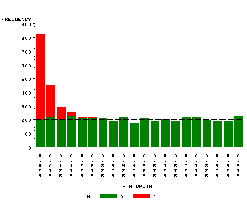
\epsfig{
% %       file=.../Figures/HistoPvalRef.ps,
% %       height=8cm, width=8cm, bbllx=82, bblly=304, bburx=277,
% %       bbury=460, angle=90, clip=} 
%   \end{tabular}
% \end{tabular}
% \paragraph{Decision rule:}
% reject $\Hbf_0$ for all $(i)$ such that
% $$
% P_{(i)} \leq \frac{i \alpha^*}n \quad \Longrightarrow \quad
%     FDR \leq \frac{n_0}n \alpha^* \leq \alpha^*
% $$

% \paragraph{Benjamini \& Yakutieli (01):} For correlated
% test statistics
% $$
% P_{(i)} \leq \frac{i \alpha^*}{n (\sum_j 1/j)}.
% $$


%%%%%%%%%%%%%%%%%%%%%%%%%%%%%%%%%%%%%%%%%%%%%%%%%%%%%%%%%%%%%%%%%%%%%%
%%%%%%%%%%%%%%%%%%%%%%%%%%%%%%%%%%%%%%%%%%%%%%%%%%%%%%%%%%%%%%%%%%%%%%
\newpage
\chapter{Local False Discovery Rate}
%%%%%%%%%%%%%%%%%%%%%%%%%%%%%%%%%%%%%%%%%%%%%%%%%%%%%%%%%%%%%%%%%%%%%%
%%%%%%%%%%%%%%%%%%%%%%%%%%%%%%%%%%%%%%%%%%%%%%%%%%%%%%%%%%%%%%%%%%%%%%

% \noindent FDR provides a general information about the risk of the whole
% procedure (up to step $i$). But we are actually interested in a
% specific risk, associated to each gene.

% \paragraph{Derivative of the FDR:} $\lFDR_{(i)}$ can be also defined as the
% derivative of the FDR
% $$
% \lFDR(t) = \lim_{h \downarrow 0} \frac{FDR(t+h) - FDR(t)}{h}
% $$
% which can be estimated by 
% $$
% \widehat{n}_0 (P_{(i)} - P_{(i-1)})
% $$
% (Aubert \& al., BMC Bioinfo., 04).

% \paragraph{Local FDR ($\lFDR$).} First defined by Efron \&
% al. (JASA, 2001) in a mixture model framework:
% $$
% \lFDR_i := \Pr\{\Hbf_0(i) \mbox{ is false} \;|\; T_i\}.
% $$


% %%%%%%%%%%%%%%%%%%%%%%%%%%%%%%%%%%%%%%%%%%%%%%%%%%%%%%%%%%%%%
% \newpage
\bigskip
\section{Semi-parametric mixture modeling} 

\paragraph{Property of the test statistic.} The standard hypotheses
testing theory implies that, under $\Hbf_0(i)$, $P_i$ is uniformly
distributed over $[0, 1]$: \\
\begin{tabular}{cc}
  \begin{tabular}{p{13.5cm}}
    $$
    P_i \underset{\Hbf_0(i)}{\sim} \Ucal_{[0, 1]}
    $$
    \\
    ~\\
    The $P_i$'s are distributed according to a mixture distribution
    with density 
    $$
    g(p) = a f(p) + (1-a) 
    $$
    \\
    The problem is then to estimate
  \end{tabular}
  &
  \begin{tabular}{c}
  \epsfig{figure=/RECHERCHE/EXPRESSION/EXPOSES/Figures/HistoPvalRef.ps, height=8cm, width=8cm,
    clip=, bbllx=26, bblly=40, bburx=176, bbury=130}   
%     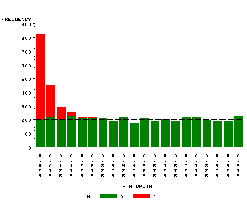
\epsfig{
%       file=.../Figures/HistoPvalRef.ps,
%       height=8cm, width=8cm, bbllx=82, bblly=304, bburx=277,
%       bbury=460, angle=90, clip=} 
  \end{tabular}
\end{tabular}
$$
\begin{tabular}{ll}
  \paragraph{$a$:} & the proportion of differentially expressed genes
  \\
  \paragraph{$f$:} & the  (alternative) density $f$ \\ 
\end{tabular}
$$

\newpage
\paragraph{Generalization:} We consider an i.i.d. sample $\{X_1,
\dots, X_n\}$ with mixture density
$$
g(x) = a f(x) + (1-a) \phi(x)
$$
\begin{tabular}{lr}
  The proportion $a$ is unknown &  $\longrightarrow$ \paragraph{parametric part} \\ 
  \\
  The density $f$ is completely unknown & \quad $\longrightarrow$ \paragraph{non
    parametric part} \\ 
  \\
  The density $\phi$ in completely specified & ($\Ucal_{[0, 1]}$,
  $\Ncal(0, 1)$, {\it etc.})
\end{tabular}

\bigskip \bigskip
\paragraph{Posterior probability.} We are interested in the
estimation of 
$$
\tau_i = \Pr\{\mbox{gene $i$ is a true positive given the data}\}
$$
that is
$$
%\tau_i = \Pr\{Z_i = 1 \;|\; x_i\} = \Esp(Z_i \;|\; x_i) = \frac{a
%  f(x_i)}{g(x_i)}
\tau_i = \Pr\{\mbox{gene $i$ comes frome distribution $f$} \;|\; x_i\}  = \frac{a
  f(x_i)}{g(x_i)}
$$
% where $Z_i =
% \left\{
% \begin{tabular}{rll}
%   $Z_i = 1$ & if $i$ comes from $f$ & ($\Hbf_0(i)$ false), \\
%   \\
%   $Z_i = 0$ & otherwise & ($\Hbf_0(i)$ true).
% \end{tabular}
% \right.$

%%%%%%%%%%%%%%%%%%%%%%%%%%%%%%%%%%%%%%%%%%%%%%%%%%%%%%%%%%%%%%%%%%%%%%
\newpage
\subsection{A trick}
%%%%%%%%%%%%%%%%%%%%%%%%%%%%%%%%%%%%%%%%%%%%%%%%%%%%%%%%%%%%%%%%%%%%%%

Perform a transformation which zooms in the left tail of the
distribution, where the red data are expected to be.

\paragraph{Probit transform.} \\
%Instead of modeling the distribution of the $P_i$', we consider the
$$
                                %\hspace{-.5cm}
\begin{tabular}{lcr}
  $P_i \in [0, 1]$
  &   
  \qquad 
  &
  $X_i = \Phi^{-1}(P_i) \in \Rbb$ 
  \\
%  \multicolumn{3}{c}{(Efron, JASA, 2005)}
  \\
  \textred{$\phi = \Ucal_{[0; 1]}$}
  & 
  & 
  \textred{$\phi = \Ncal(0, 1)$}
  \\
  \\
  \epsfig{figure=/Recherche/Expression/Exposes/Figures/HistoPval.ps,
  height=8cm, width=11.5cm, clip=, bbllx=26, bblly=40, bburx=176,
  bbury=130}    
  &
  &
%  \vspace{-2cm}
  \epsfig{figure=/Recherche/Expression/Exposes/Figures/HistoProbit.ps,
    height=8cm, width=11.5cm, clip=, bbllx=26, bblly=39, bburx=176,
    bbury=130}    
\end{tabular}
$$

%%%%%%%%%%%%%%%%%%%%%%%%%%%%%%%%%%%%%%%%%%%%%%%%%%%%%%%%%%%%%%%%%%%%%%
\newpage
\section{Hedenfalk data}

% \paragraph{Student t-test} with homogenous variance $\sigma_g = $
% cst. Gaussian kernel.

% \hspace{-2cm}
% \begin{tabular}{cc} 
%   \begin{tabular}{c}
%     $\widehat{a} = 20.6 \%$ \\
%     $\textblue{\widehat{g}(x)}  = \widehat{a} \textred{\widehat{f}(x)} + (1-\widehat{a})
%     \textgreen{\phi(x)}$ \\ 
%     \epsfig{
%       file=/RECHERCHE/EXPRESSION/EXEMPLES/HEDENFALK/Ainit/Asup-1.0/Homogen-Gaus.eps,
%       height=12cm, width=9cm, bbllx=66, bblly=510, bburx=283,
%       bbury=691, clip=, angle=90} 
%   \end{tabular}
%   &
%   \begin{tabular}{c} 
%     $\textred{\widehat{FDR}_i}, \textblue{\widehat{\tau}_i} \times
%     \Phi^{-1}(P_i)$ \\ 
%     \epsfig{
%       file=/RECHERCHE/EXPRESSION/EXEMPLES/HEDENFALK/Ainit/Asup-1.0/Homogen-Gaus.eps,
%       height=12cm, width=4.5cm, bbllx=66, bblly=295, bburx=283,
%       bbury=480, clip=, angle=90} 
%     \\
%     $\textred{\widehat{FDR}_i}, \textblue{\widehat{\tau}_i} \times
%     P_i$ \\ 
%     \epsfig{
%       file=/RECHERCHE/EXPRESSION/EXEMPLES/HEDENFALK/Ainit/Asup-1.0/Homogen-Gaus.eps,
%       height=12cm, width=4.5cm, bbllx=66, bblly=85, bburx=283,
%       bbury=265, clip=, angle=90} 
%   \end{tabular}
% \end{tabular}

% \noindent $\Hbf_0$ (negative) $p$-values are not uniformly distributed
% over [0, 1]. \\
% The non-parametric part $\widehat{f}$ captures this departure of the
% null distribution.

% \newpage
%
\hspace{-2cm}
\begin{tabular}{cc} 
  \begin{tabular}{c}
    $\widehat{a} = 30.5 \%$ \\
    $\textblue{\widehat{g}(x)}  = a \textred{\widehat{f}(x)} + (1-a)
    \textgreen{\phi(x)}$ \\ 
    \epsfig{
      file=/RECHERCHE/EXPRESSION/EXEMPLES/HEDENFALK/Ainit/Asup-1.0/Varmixt-Gaus.eps,
      height=12cm, width=9cm, bbllx=66, bblly=510, bburx=283,
      bbury=691, clip=, angle=90} 
  \end{tabular}
  &
  \begin{tabular}{c} 
    $\textred{\widehat{FDR}_i}, \textblue{\widehat{\tau}_i} \times
    \Phi^{-1}(P_i)$ \\ 
    \epsfig{
      file=/RECHERCHE/EXPRESSION/EXEMPLES/HEDENFALK/Ainit/Asup-1.0/Varmixt-Gaus.eps,
      height=12cm, width=4.5cm, bbllx=66, bblly=295, bburx=283,
      bbury=480, clip=, angle=90} 
    \\
    $\textred{\widehat{FDR}_i}, \textblue{\widehat{\tau}_i} \times
    P_i$ \\ 
    \epsfig{
      file=/RECHERCHE/EXPRESSION/EXEMPLES/HEDENFALK/Ainit/Asup-1.0/Varmixt-Gaus.eps,
      height=12cm, width=4.5cm, bbllx=66, bblly=85, bburx=283,
      bbury=265, clip=, angle=90} 
  \end{tabular}
\end{tabular}

\centerline{$
  \begin{array}{ccccc}
    \quad \widehat{FDR}_{(i)} \quad & \qquad i \qquad & \quad P_{(i)}
    \quad & \quad \widehat{\tau}_{(i)} \quad & \quad
    \widehat{FNR}_{(i)} \quad \\  
    \hline
    1\% & 4 & 2.5\;10^{-5} & 0.988 & 31.5 \% \\
    5\% & 142 & 3.1\;10^{-3} & 0.914 & 28.7 \% \\
    10\% & 296 & 1.3\;10^{-2} & 0.798 & 25.7 \% \\
  \end{array}
$}
\vspace{-0.5cm}
$\widehat{FDR}_{(i)} = \widehat{FNR}_{(i)} = 19.7 \%$ for $(i) = 633,
P_{(i)} = 5.4 \%, \widehat{\tau}_{(i)} = 43.5 \%$.

%%%%%%%%%%%%%%%%%%%%%%%%%%%%%%%%%%%%%%%%%%%%%%%%%%%%%%%%%%%%
\newpage
\subsection{Possible extension to ChIP-chip data?}

\paragraph{Aim.} Detect binding sites of a given transcription factor.

\paragraph{Distribution of the signal.} We expect 2 populations:
hybridized / non-hybridized $\rightarrow$ same kind of situation.

\paragraph{But...} the modeling does not seem that easy:
$$
\begin{tabular}{cc}
  Raw data & Mixture model \\
  \epsfig{figure=../../ChIP-Chip/URGV-1005/Fig-ResNormOK-dif-Histo.eps,
    angle = 90, height = 8cm, clip=}
  &
  \epsfig{figure=../../ChIP-Chip/URGV-1005/Fig-ResNormOK-dif-Agregate.eps, 
    angle = 90, height = 8cm, clip=}
\end{tabular}
$$

% %%%%%%%%%%%%%%%%%%%%%%%%%%%%%%%%%%%%%%%%%%%%%%%%%%%%%%%%%%%%
% \newpage
% \subsection{Semi-parametric mixture modeling}

% \paragraph{Alternative point of view.} The genes may belong to 2
% populations:
% \begin{enumerate}
% \item \vspace{-0.75cm} The 'null' population (proportion $1-a$) for which
%   the distribution $\phi$ of the test statistic is known.
% \item \vspace{-0.75cm} The 'positive' population (proportion $a$) for
%   which the distribution $f$ of the test statistic is unknown.
% \end{enumerate}
% We would like to know the probability $\tau_i$ for gene $i$ to belong
% to the 'positive' population. 
% $$
% \begin{tabular}{cc} 
%   $\wto observe idehat{a} = 30.5 \%$ \\
%   \begin{tabular}{c}
%     $\textblue{\widehat{g}(x)}  = \widehat{a} \textred{\widehat{f}(x)} + (1-\widehat{a})
%     \textgreen{\phi(x)}$ \\ 
%     \epsfig{
%       file=/RECHERCHE/EXPRESSION/EXEMPLES/HEDENFALK/Ainit/Asup-1.0/Varmixt-Gaus.eps,
%       height=10cm, width=7cm, bbllx=66, bblly=510, bburx=283,
%       bbury=691, clip=, angle=90} 
%   \end{tabular}
%   &
%   \begin{tabular}{c} 
%     $\textred{\widehat{FDR}_i}, \textblue{\widehat{\tau}_i} \times
%     \Phi^{-1}(P_i)$ \\ 
%     \epsfig{
%       file=/RECHERCHE/EXPRESSION/EXEMPLES/HEDENFALK/Ainit/Asup-1.0/Varmixt-Gaus.eps,
%       height=10cm, width=7cm, bbllx=66, bblly=295, bburx=283,
%       bbury=480, clip=, angle=90} 
%   \end{tabular}
% \end{tabular}
% $$
% % \centerline{$
% %   \begin{array}{ccccc}
% %     \quad \widehat{FDR}_{(i)} \quad & \qquad i \qquad & \quad P_{(i)}
% %     \quad & \quad \widehat{\tau}_{(i)} \quad & \quad
% %     \widehat{FNR}_{(i)} \quad \\  
% %     \hline
% %     1\% & 4 & 2.5\;10^{-5} & 0.988 & 31.5 \% \\
% %     5\% & 142 & 3.1\;10^{-3} & 0.914 & 28.7 \% \\
% %     10\% & 296 & 1.3\;10^{-2} & 0.798 & 25.7 \% \\
% %   \end{array}
% % $}
% % \vspace{-0.5cm}
% % $\widehat{FDR}_{(i)} = \widehat{FNR}_{(i)} = 19.7 \%$ for $(i) = 633,
% % P_{(i)} = 5.4 \%, \widehat{\tau}_{(i)} = 43.5 \%$.

% %%%%%%%%%%%%%%%%%%%%%%%%%%%%%%%%%%%%%%%%%%%%%%%%%%%%%%%%%%%%%
% %%%%%%%%%%%%%%%%%%%%%%%%%%%%%%%%%%%%%%%%%%%%%%%%%%%%%%%%%%%%%
% % \newpage
% % \chapter{Mixture model for Chip-chip data}
% % %%%%%%%%%%%%%%%%%%%%%%%%%%%%%%%%%%%%%%%%%%%%%%%%%%%%%%%%%%%%%
% % %%%%%%%%%%%%%%%%%%%%%%%%%%%%%%%%%%%%%%%%%%%%%%%%%%%%%%%%%%%%%

% % \paragraph{Raw data.}
% % $$
% % \epsfig{figure=../../ChIP-Chip/URGV-1005/Fig-ResNormOK-dif-Histo.eps, 
% %   angle = 90, height = 10cm, clip=}
% % $$


% % %%%%%%%%%%%%%%%%%%%%%%%%%%%%%%%%%%%%%%%%%%%%%%%%%%%%%%%%%%%%%
% % \newpage
% % \begin{tabular}{cc}
% %   {\small% %     \epsfig{figure=../../ChIP-Chip/URGV-1005/Fig-ResNormOK-dif-Agregate.eps, 
% %       angle = 90, height = 8cm, clip=}

% %     $\begin{array}{ccc}
% %       \widehat{\pi}_k (\%) & \widehat{\mu}_k & \widehat{\sigma}_k \\
% %       \hline
% %       0.8 & -1.19 & 1.37 \\ 
% %       8.2 & -1.11 & 0.76 \\ 
% %       31.3 & -0.52 & 0.48 \\ 
% %       23.6 & 0.04 & 0.20 \\ 
% %       18.8 & 0.38 & 0.46 \\ 
% %       \hline
% %       9.9 & 1.28 & 0.63 \\ 
% %       \hline
% %       0.8 & 1.42 & 1.33 \\ 
% %       6.6 & 2.45 & 0.68 \\ 
% %     \end{array}$
% %     }
% %     & 
% %     \begin{tabular}{c}
% %       \epsfig{figure=../../ChIP-Chip/URGV-1005/Fig-ResNormOK-dif-Mixture.eps, 
% %         angle = 90, height = 10cm, clip=}
% %     \end{tabular}
% % \end{tabular}

% % %%%%%%%%%%%%%%%%%%%%%%%%%%%%%%%%%%%%%%%%%%%%%%%%%%%%%%%%%%%%%
% % \newpage
% % \begin{tabular}{cc}
% %   \begin{tabular}{c}
% %     \epsfig{figure=../../ChIP-Chip/URGV-1005/Fig-ResNormOK-dif-Agregate.eps, 
% %       angle = 90, height = 8cm, clip=}
% %   \end{tabular}
% %   & 
% %   \begin{tabular}{c}
% %     \epsfig{figure=../../ChIP-Chip/URGV-1005/Fig-ResNormOK-dif-Posterior.eps, 
% %       angle = 90, height = 8cm, clip=}
% %   \end{tabular}
% % \end{tabular}

%%%%%%%%%%%%%%%%%%%%%%%%%%%%%%%%%%%%%%%%%%%%%%%%%%%%%%%%%%%%%
%%%%%%%%%%%%%%%%%%%%%%%%%%%%%%%%%%%%%%%%%%%%%%%%%%%%%%%%%%%%%
\newpage
\chapter{Segmentation-clustering for CGH array} 
%%%%%%%%%%%%%%%%%%%%%%%%%%%%%%%%%%%%%%%%%%%%%%%%%%%%%%%%%%%%%
%%%%%%%%%%%%%%%%%%%%%%%%%%%%%%%%%%%%%%%%%%%%%%%%%%%%%%%%%%%%%

%%%%%%%%%%%%%%%%%%%%%%%%%%%%%%%%%%%%%%%%%%%%%%%%%%%%%%%%%%%%%
\bigskip
\subsection{CGH microarray technology in its principle }
%%%%%%%%%%%%%%%%%%%%%%%%%%%%%%%%%%%%%%%%%%%%%%%%%%%%%%%%%%%%%
$$
\epsfig{file = ../Figures/principe_CGH.eps, clip=,
  bbllx=0, bblly=41, bburx=700, bbury=478, scale=0.9}
$$

%%%%%%%%%%%%%%%%%%%%%%%%%%%%%%%%%%%%%%%%%%%%%%%%%%%%%%%%%%%%%
\newpage
\subsection{Interpretation of a CGH profile }
%%%%%%%%%%%%%%%%%%%%%%%%%%%%%%%%%%%%%%%%%%%%%%%%%%%%%%%%%%%%%
\vspace{-0.5cm}
$$
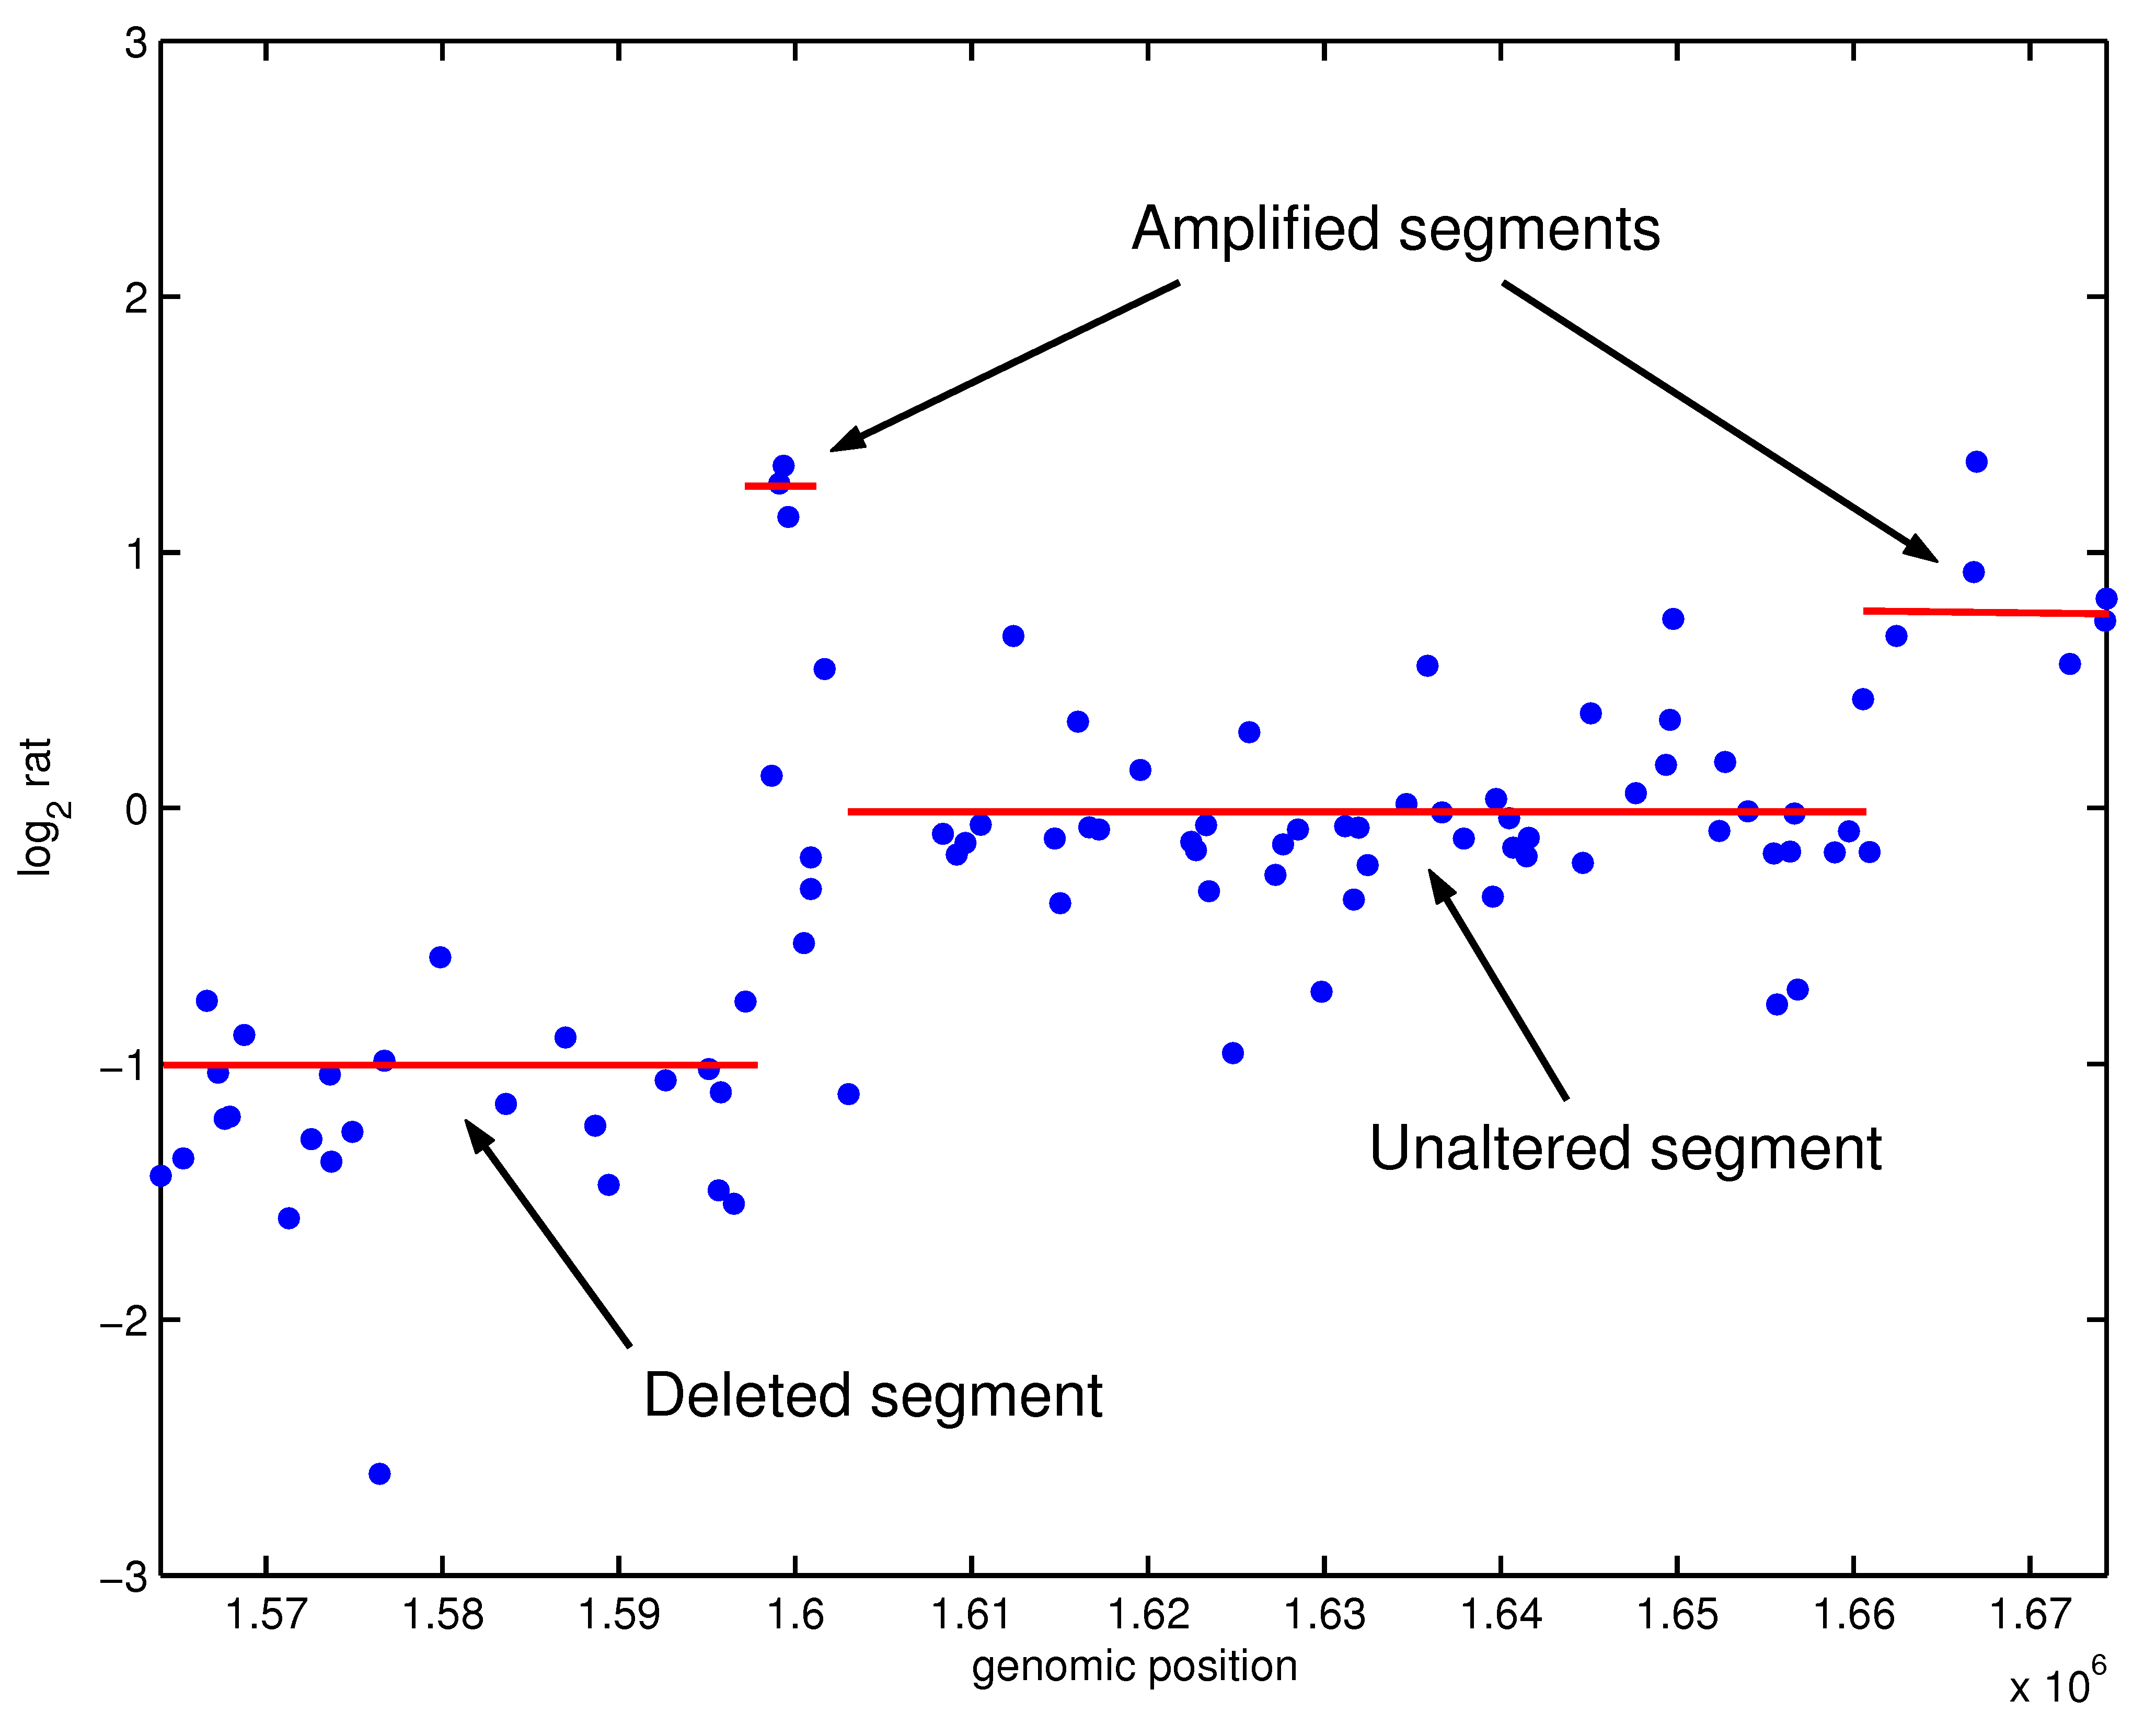
\epsfig{file = ../Figures/profile_example.eps, clip=,
  bbllx=60, bblly=196, bburx=543, bbury=586}
$$
\centerline{
  A dot on the graph 
  $
  \displaystyle{
    = \log_2 \left\{ \frac{\text{ $\sharp$ copies of BAC(t) in the test
          genome }}{\text{$\sharp$ copies of BAC(t) in the reference
          genome}}\right\}}
  $
}

%%%%%%%%%%%%%%%%%%%%%%%%%%%%%%%%%%%%%%%%%%%%%%%%%%%%%%%%%%
%%%%%%%%%%%%%%%%%%%%%%%%%%%%%%%%%%%%%%%%%%%%%%%%%%%%%%%%%%
\newpage
\section{A first modeling}
%%%%%%%%%%%%%%%%%%%%%%%%%%%%%%%%%%%%%%%%%%%%%%%%%%%%%%%%%%
%%%%%%%%%%%%%%%%%%%%%%%%%%%%%%%%%%%%%%%%%%%%%%%%%%%%%%%%%%

%%%%%%%%%%%%%%%%%%%%%%%%%%%%%%%%%%%%%%%%%%%%%%%%%%%%%%%%%%
\bigskip
\subsection{Break-points detection in a signal} 
\begin{itemize}
\item $Y_t =$ (random) log-ratio measured for the BAC number $t$.
\item The mean (and variance) of $Y_t$ changes at $(K-1)$ unknown
  coordinates $T=(t_1, ..., t_{K-1})$ ($\Rightarrow K$ segments).
\item The parameters of this model are: 
  \begin{eqnarray*}
    \mbox{the break point positions:} & T = & (t_1, ..., t_{K-1}), \\
    \\
    \mbox{the mean (and variance)} & & \\
    \mbox{of the log-ratio in each segment:} &
    \Theta = & (\mu_1, \sigma_1^2; \hdots; \mu_K,\sigma_K^2).
    \end{eqnarray*}
\end{itemize}
Break-points detection aims at studying the \textblue{spatial
    structure of the signal}.


%%%%%%%%%%%%%%%%%%%%%%%%%%%%%%%%%%%%%%%%%%%%%%%%%%%%%%%%%%
\newpage
%\subsection{Estimating the parameters in a model of abrupt-changes detection}
%%%%%%%%%%%%%%%%%%%%%%%%%%%%%%%%%%%%%%%%%%%%%%%%%%%%%%%%%%

% \paragraph{Estimating the parameters with $K$ fixed by maximum likelihood}
% \begin{itemize}
% \item Joint estimation of $T$ and $\Theta$ with dynamic programming.
% \item Dynamic programming works because the log-ratios are assumed to
%   be independent (at least from one segment to another).
% \end{itemize}

% % \paragraph{Log-Likelihood} 
% % $$
% % \Lcal_K(T, \Theta)= \sum_{k=1}^K \log f(y^k;
% % \theta_k)=\sum_{k=1}^K \sum_{t \in I_k}\log f(y_t; \theta_k)
% % $$
% \paragraph{Model Selection: choice of $K$}
% \begin{itemize}
% \item The fit of the modelling is measured by the likelihood of the
%   data given the estimated parameters: $\Lcal_K$
% \item Penalized Likelihood: 
%   $$
%   \hat{K} = \underset{K}{\arg\max}\left( \hat{\Lcal}_K - \beta K \right).
%   $$
% \item The parameter $\beta$ can be fixed, estimated or used as a
%   tuning parameter.
% \end{itemize}

%%%%%%%%%%%%%%%%%%%%%%%%%%%%%%%%%%%%%%%%%%%%%%%%%%%%%%%%%%
\newpage
\subsection{Example of segmentation on array CGH data}
%%%%%%%%%%%%%%%%%%%%%%%%%%%%%%%%%%%%%%%%%%%%%%%%%%%%%%%%%%

\paragraph{Are the variances $\sigma^2_k$ homogeneous?} BT474 cell
line, chromosome 9: 
$$
\begin{tabular}{cc}
  Homogeneous variances & Heterogeneous variances \\
  \multicolumn{2}{c}{$K=4$ segments} \\
  \epsfig{file = ../Figures/bt474_c9_seg_homo_K4.eps, clip=, scale=0.7} &
  \epsfig{file = ../Figures/bt474_c9_seg_hetero_K4.eps, clip=, scale=0.7} \\
\end{tabular}
$$

%%%%%%%%%%%%%%%%%%%%%%%%%%%%%%%%%%%%%%%%%%%%%%%%%%%%%%%%%%
\newpage
\paragraph{Adaptive choice of the number of segments.} BT474 cell
line, chromosome 1:
$$
\begin{tabular}{cc}
  Homogeneous variances & Heterogeneous variances \\
  $\widehat{K} = 10$  segments & $\widehat{K} = 2$ segments \\
  \epsfig{file = ../Figures/bt474_c1_seg_homo_K10.eps, clip=, scale=0.7} &
  \epsfig{file = ../Figures/bt474_c1_seg_hetero_K2.eps, clip=, scale=0.7} \\
\end{tabular}
$$
Homogeneous variances result in smaller segments.

% %%%%%%%%%%%%%%%%%%%%%%%%%%%%%%%%%%%%%%%%%%%%%%%%%%%%%%%%%
% \newpage
% \subsection{Comparative study} 

% \paragraph{Lai \& al. (Bioinformatics, 05).} On both synthetic and
% real data (GBM brain tumor data), our method 'CGHseg' performs well.
% $$
% %\epsfig{file = ../Figures/LPJ05-Fig1.eps, clip=, scale=1.2}
% %\epsfig{file = ../Figures/LPJ05-Fig3.eps, clip=, scale=1.2}
% \epsfig{file = ../Figures/LPJ05-Fig4.eps, clip=, scale=1.2}
% $$


% %%%%%%%%%%%%%%%%%%%%%%%%%%%%%%%%%%%%%%%%%%%%%%%%%%%%%%%%%%
% \newpage
% \paragraph{ROC curves.} The sensitivity decreases for small segments
% when  signal-to-noise ratio (SNR) is small.
% $$
% \epsfig{file = ../Figures/LPJ05-Fig2.eps, clip=, scale=1.2}
% $$

%%%%%%%%%%%%%%%%%%%%%%%%%%%%%%%%%%%%%%%%%%%%%%%%%%%%%%%%%%
%%%%%%%%%%%%%%%%%%%%%%%%%%%%%%%%%%%%%%%%%%%%%%%%%%%%%%%%%%
\newpage
\section{A new model for segmentation-clustering}
%%%%%%%%%%%%%%%%%%%%%%%%%%%%%%%%%%%%%%%%%%%%%%%%%%%%%%%%%%
%%%%%%%%%%%%%%%%%%%%%%%%%%%%%%%%%%%%%%%%%%%%%%%%%%%%%%%%%%

\bigskip
\paragraph{Considering the biological problem and the need for a new
  model.}  
$$
\begin{tabular}{cc}
  \epsfig{file = ../Figures/FigSegClas-1.eps, clip=, scale=0.7} &
  \epsfig{file = ../Figures/FigSegClas-2.eps, clip=, scale=0.7} \\
\end{tabular}
$$
We'd like segments of same type ('normal', 'deleted', amplified',
{\it etc.}) to be gathered into groups.
% $$
% \epsfig{file = ../Figures/nouveau_modele.ps, angle=270, clip=,
%   bbllx=92, bblly=47, bburx=484, bbury=828, scale=0.9}
% $$

%%%%%%%%%%%%%%%%%%%%%%%%%%%%%%%%%%%%%%%%%%%%%%%%%%%%%%%%%%
\newpage
\paragraph{Mixture model for segments:} 
\begin{itemize}
\item We suppose there exists a \textblue{secondary underlying
    structure} of the segments into $P$ populations:
  $$
  \pi_p = \mbox{proportion of group $p$}
%   (Z_{k1},\hdots,Z_{kP}) \sim \mathcal{M}(1;\pi_1,\hdots,\pi_P).
  $$
\item Conditionally to the group to which the segment belongs, we know
  the distribution of $Y$:
  $$
  \mbox{BAC } t \mbox{ belongs to a segment of group } p \quad
  \Rightarrow \quad Y_t \mbox{ has mean } m_p \mbox{ (and variance } s_p^2).
%   Y^k|Z_{kp}=1 \sim \Ncal({\bf 1}_{n_k} m_p, s_p^2 {\bf I}_{n_k}).
  $$
%\item It is a model of \textblue{segmentation/clustering}.
\item The parameters of this model are
  \begin{eqnarray*}
    \mbox{the brakpoint positions:} \quad T&=&(t_1, ..., t_{K-1}),\\
    \mbox{the mixture characteristics:} \quad
    \Theta&=&(\pi_1,\hdots,\pi_P;m_1, \hdots, m_P; s_1^2, \hdots ,s_P^2).
  \end{eqnarray*}
\end{itemize}

% %%%%%%%%%%%%%%%%%%%%%%%%%%%%%%%%%%%%%%%%%%%%%%%%%%%%%%%%%%
% \newpage
% \section{Likelihood and statistical units of the model }
% %%%%%%%%%%%%%%%%%%%%%%%%%%%%%%%%%%%%%%%%%%%%%%%%%%%%%%%%%%


% \vspace{-0.5cm}    \mbox{the brakpoint positions:} \quad 
% \begin{itemize}
% \item the statistical units are segments:$Y^k$,
% \item the density of $Y^k$ is a mixture density:
%   $$
%   \log \Lcal_{KP}(T, \Theta)= \sum_{k=1}^K \log
%   f(y^k;\Theta)=\sum_{k=1}^K \log \left\{ \sum_{p=1}^P \pi_p
%     f(y^k;\theta_p) \right\}
%   $$
% \item \vspace{-0.5cm} If the $Y_ts$ are independent, we have:
%   $$
%   \log \Lcal_{KP}(T,\Theta) =\textcolor{red}{\sum_{k=1}^K} \log
%   \left\{ \textcolor{blue}{\sum_{p=1}^P} \pi_p \textcolor{red}{\prod_{
%         t \in I_k }}f(y_t; \theta_p) \right\}. 
%   $$
%   instead of $ \log \Lcal_{P}(\Theta) =
%   \textcolor{red}{\sum_{k=1}^K} \log \left\{ \textcolor{red}{\prod_{ t
%         \in I_k }} \textcolor{blue}{\sum_{p=1}^P} \pi_p f(y_t;
%     \theta_p)\right \} $ in the classical mixture model where the
%   statistical units are the elementary data $Y_t$s.
% \end{itemize}

%%%%%%%%%%%%%%%%%%%%%%%%%%%%%%%%%%%%%%%%%%%%%%%%%%%%%%%%%%
\newpage
\subsection{An hybrid estimation algorithm}
%%%%%%%%%%%%%%%%%%%%%%%%%%%%%%%%%%%%%%%%%%%%%%%%%%%%%%%%%%

\paragraph{Alternate parameters estimation with $K$ and $P$ known}
\begin{enumerate}
\item When $T$ is fixed, the \textblue{Expectation-Maximisation (EM)}
  algorithm estimates $\Theta$:
  $$
  T = (t_1, \dots, t_{K-1}) \quad \rightarrow \quad \Theta =
  (\pi_1,\hdots,\pi_P;m_1, \hdots, m_P; s_1^2, \hdots ,s_P^2)
  $$
\item When $\Theta$ is fixed, \textblue{dynamic programming} estimates $T$:
  $$
  \Theta = (\pi_1,\hdots,\pi_P;m_1, \hdots, m_P; s_1^2, \hdots
  ,s_P^2) \quad \rightarrow \quad T = (t_1, \dots, t_{K-1})
  $$
\end{enumerate} 

\paragraph{An increasing sequence  of likelihoods:}
At each step (1 or 2), the likelihood increases 
$$
\Rightarrow \mbox{ the algorithm converges}.
$$

% %%%%%%%%%%%%%%%%%%%%%%%%%%%%%%%%%%%%%%%%%%%%%%%%%%%%%%%%%%
% \newpage
% \subsection{Mixture Model when the segmentation is known}
% %%%%%%%%%%%%%%%%%%%%%%%%%%%%%%%%%%%%%%%%%%%%%%%%%%%%%%%%%%

% \paragraph{Mixture model parameters estimators.}
% \begin{eqnarray}
% \mbox{posterior probability:} \qquad \hat{\tau}_{kp} & = & \frac{\hat{\pi}_p f(y^k; \hat{\theta}_p)}{\suml \hat{\pi}_{\ell} f(y^k; \hat{\theta}_{\ell})}. \nonumber
% \end{eqnarray}
% \begin{itemize}
% \item the estimator the the mixing proportions is: $\hat{\pi}_p = \frac{\sumtau}{K}$.
% \item In the gaussian case, $\theta_p=(m_p,s_p^2)$: 
% \begin{eqnarray}
% \mbox{weighted mean:} \qquad \hat{m}_p   &=&  \frac{\sumtau \sumt y_t}{\sumtau n_k}, \nonumber \\
% \mbox{weighted variance:} \qquad \hat{s}_p^2 &=&  \frac{\sumtau \sumt (y_t- \hat{m}_p)^2}{\sumtau n_k}. \nonumber 
% \end{eqnarray}
% \item Big size vectors will have a bigger impact in the estimation of the parameters, via the term $\sumtau n_k$ \\
% \end{itemize}

% %%%%%%%%%%%%%%%%%%%%%%%%%%%%%%%%%%%%%%%%%%%%%%%%%%%%%%%%%%
% \newpage
% \subsection{Segmentation with a fixed mixture}
% %%%%%%%%%%%%%%%%%%%%%%%%%%%%%%%%%%%%%%%%%%%%%%%%%%%%%%%%%%

% \paragraph{Back to dynamic programming}
% \begin{itemize}
% \item the incomplete mixture log-likelihood can be written as a sum of local log-likelihoods:
%   $$
%   \begin{array}{ccccc}
%     \Lcal_{KP}(T,\Theta) & = & \sumk \ell_{kP}(y^k;\Theta) 
%   \end{array}
%   $$
% \item the local log-likelihood of segment $k$ corresponds to the
%   mixture log-density of vector $Y^k$
%   $$
%   \ell_{kP}(y^k;\Theta)=\log \left\{\sum_{p=1}^P \pi_p \prod_{t \in
%       I_k} f(y_t;\theta_p)\right\}.
%   $$
% \item $\log \Lcal_{KP}(T,\Theta)$ can be optimized in $T$ with $\Theta$ fixed, by dynamix programming. 
% \end{itemize}

% %%%%%%%%%%%%%%%%%%%%%%%%%%%%%%%%%%%%%%%%%%%%%%%%%%%%%%%%%%%
% \newpage
% \subsection{Model selection: $K=?$, $P=?$}
% %%%%%%%%%%%%%%%%%%%%%%%%%%%%%%%%%%%%%%%%%%%%%%%%%%%%%%%%%%%

% \paragraph{Choosing the number of groups $P$.} 

% \vspace{-0.5cm}
% We use the BIC criterion:
% $$
% BIC = \Lcal_{P} - \log n \times (\# \mbox{ of parameters}) / 2
% $$
% \vspace{-1cm}
% $$
% \begin{tabular}{cc}
%   Simulated sequence & $\Lcal_{KP}$ and $BIC$ criterion \\
%   \epsfig{file = ../Figures/Exemple_P2K4.eps, clip=, scale=0.7} &
%   \epsfig{file = ../Figures/Exemple_P2K4_BIC.eps, clip=, scale=0.7} \\
% \end{tabular}
% $$
% The log-likelihood $\Lcal$ (\textred{\bf ---}) always increases with
% $P$ while $BIC$ ({\bf ---}) has a maximum.

% %%%%%%%%%%%%%%%%%%%%%%%%%%%%%%%%%%%%%%%%%%%%%%%%%%%%%%%%%%%
% \newpage
% \paragraph{Choosing the number of segments $K$.} 

% The likelihood may decrease when $K$ increases:
% $$
% \begin{tabular}{lc}
%   \hspace{-1cm}
%   \begin{tabular}{l}
%     Simulated data: \\
%     \\
%     $f(y^k;\Theta) =$ \\
%     \\
%     $0.5 \Ncal(0,1)+ 0.5 \Ncal(5,1)$ \\
%     \\
%     \\
%     Log-likelihood $\Lcal_{KP}$ \\
%     as a function of $K$ \\
%     \\
%     ($P=2$) \\
%     \\
%   \end{tabular}
%   & \begin{tabular}{c}
%     \epsfig{file = ../Figures/simulation_2.eps, clip=, scale=0.8}
%   \end{tabular}
% \end{tabular}
% $$
% $\rightarrow$ sort of self-penalization of the log-likelihood with
% respect to $K$.

%%%%%%%%%%%%%%%%%%%%%%%%%%%%%%%%%%%%%%%%%%%%%%%%%%%%%%%%%%%
\newpage
\subsection{Example: CGH for BT474 cell line}
%%%%%%%%%%%%%%%%%%%%%%%%%%%%%%%%%%%%%%%%%%%%%%%%%%%%%%%%%%%

\paragraph{Interest of clustering: an easy case.} \\
Chromosome 9:
$$
  \begin{tabular}{cc}
    Segmentation & Segmentation/Clustering \\
    \multicolumn{2}{c}{$K=4$ segments} \\
    \epsfig{file = ../Figures/bt474_c9_seg_homo_K4, clip=, scale=0.7} 
    & 
    \epsfig{file = ../Figures/bt474_c9_segclas_homo_P3K4 , clip=, scale=0.7} 
  \end{tabular}
$$
Clustering defines 'deleted', 'normal' and 'amplified' groups.

\newpage

\paragraph{Interest of clustering: a more interesting case.} \\
Chromosome 1:
$$
\begin{tabular}{cc}
  Segmentation & Segmentation/Clustering \\
  $K=2$ & $P=3$, $K=8$ \\
  \epsfig{file = ../Figures/bt474_c1_seg_hetero_K2.eps, clip=, scale=0.7} 
  & \epsfig{file = ../Figures/resultat_P3K8.eps , clip=, scale=0.7} 
\end{tabular}
$$
Clustering detects an outliers and captures a 'normal' segment within
a large variance region.


% %%%%%%%%%%%%%%%%%%%%%%%%%%%%%%%%%%%%%%%%%%%%%%%%%%%%%%%%%%%
% %%%%%%%%%%%%%%%%%%%%%%%%%%%%%%%%%%%%%%%%%%%%%%%%%%%%%%%%%%%
% \newpage
% \section{Conclusion and future works}
% %%%%%%%%%%%%%%%%%%%%%%%%%%%%%%%%%%%%%%%%%%%%%%%%%%%%%%%%%%%
% %%%%%%%%%%%%%%%%%%%%%%%%%%%%%%%%%%%%%%%%%%%%%%%%%%%%%%%%%%%

% \paragraph{What we did:}
% \vspace{-0.5cm}
% \begin{itemize}
% \item Definition of a new model that considers the \textit{a priori}
%   knowledge we have about the biological phenomena under study.
% \item Development of an hybrid algorithm (EM/dynamic programming) for
%   the parameters estimation (problems linked to EM: initializtion,
%   local maxima, degeneracy).
% \item Still waiting for an other data set to assess the performance of
%   the clustering.
% \end{itemize}

% \paragraph{What we still have to do:}
% \vspace{-0.5cm}
% \begin{itemize}
% \item Modeling: Comparison with Hidden Markov Models
% \item Model choice: Develop an adaptive procedure for two components.
% \item Other application field: DNA sequences (in progress)
% \end{itemize}


%%%%%%%%%%%%%%%%%%%%%%%%%%%%%%%%%%%%%%%%%%%%%%%%%%%%%%%%%%%%%%%%%%%%%%
%%%%%%%%%%%%%%%%%%%%%%%%%%%%%%%%%%%%%%%%%%%%%%%%%%%%%%%%%%%%%%%%%%%%%%
%%%%%%%%%%%%%%%%%%%%%%%%%%%%%%%%%%%%%%%%%%%%%%%%%%%%%%%%%%%%%%%%%%%%%%
%%%%%%%%%%%%%%%%%%%%%%%%%%%%%%%%%%%%%%%%%%%%%%%%%%%%%%%%%%%%%%%%%%%%%%
\end{document}
%%%%%%%%%%%%%%%%%%%%%%%%%%%%%%%%%%%%%%%%%%%%%%%%%%%%%%%%%%%%%%%%%%%%%%
%%%%%%%%%%%%%%%%%%%%%%%%%%%%%%%%%%%%%%%%%%%%%%%%%%%%%%%%%%%%%%%%%%%%%%
%%%%%%%%%%%%%%%%%%%%%%%%%%%%%%%%%%%%%%%%%%%%%%%%%%%%%%%%%%%%%%%%%%%%%%
%%%%%%%%%%%%%%%%%%%%%%%%%%%%%%%%%%%%%%%%%%%%%%%%%%%%%%%%%%%%%%%%%%%%%%
